\newpage
\section{The RS01 codec}
\label{rs01}
This section describes the dvdisaster RS01 Reed-Solomon codec. 
It was conceived during the summer of 2004 for creating 
error correction files in the first dvdisaster versions.
At this time, CD media was still predominant. 
Typical machines were based on Pentium 4 (tm) processors.
Measured by todays standards physical RAM and hard disk
space were scarce, and especially hard disk random I/O
was extremely slow. 

\smallskip

In order to work efficiently with the available technology,
RS01 was designed to be as space efficient as possible 
and to minimize hard disk random access. 
Optimizing the data layout for random access efficiency
lead to a parity byte distribution which left the error correction
file vulnerable to being damaged. RS01 was 
occasionally being critcized for not being able to recover 
from damaged error corrction files, but these points
were not really fair. RS01 error correction
files were never designed for being stored on fragile
media. They are supposed to
be either stored on hard disk, or to be stored on optical
media which itself is protected by dvdisaster error
correction which has the following consequences:
 Unlike optical media, hard disks do not degrade
gradually. Hard disks are usually either 100\% readable or 
completely dead, so we can assume that error correction
files on hard disk are either completely readable or fully lost.

Storing error correction files on optical media is a different
story. While an error correction file could protect itself to some
degree against lost sectors (as RS03 ecc files do), it is still
prone to the shortcomings of a file level error correction. 
The biggest disadvantage of file level error correction is
that there is no protection of file system meta data.
If meta data like a directory node becomes damaged, all files
in the directory are lost regardless of the redundancy contained
within the files. Therefore any medium containing error 
correction files must be protected with an image level
error correction layer (by using RS01,RS02 or RS03 on the medium), 
since only image level error correction avoids meta 
data sectors to become a single point of failure. See the
discussion at \url{http://dvdisaster.net/en/qa32.html} for
more information on the advantages of image level data protection
over file level approaches.

\smallskip

Nevertheless, the time has come to phase out the RS01 codec.
Consider creating an error correction file with 32 roots 
for a 650MiB sized image using both  codecs\footnote{The benchmark was
done using the GNU/Linux version 
of dvdisaster 0.79.4 on a AMD Athlon(tm) II X4 615e 
processor. RS03 used all 4 cores of the machine.
Both image and ecc files were stored in {\tt /dev/shm}
to rule out I/O effects.}:

\begin{center}
\begin{tabular}{|l|r|r|}
\hline
codec & ecc file size & encoding time \\
\hline
RS01 & 94.58MiB & 46.2s \\
RS03 & 96.68MiB &  2.4s \\
\hline
\end{tabular}
\end{center}

RS03 is about 2.2\% less storage efficient than RS01 since
its data layout has been rearranged for better parallelization.
But this is made up by a 19-fold speed improvement as
RS03 can use multiple cores and SSE2 extensions
(of course the speed improvement varies depending on the
hardware used).
Since all other properties of RS03 do at least match those
of RS01, it's fair to begin phasing out RS01 in dvdisaster.

%\smallskip

dvdisaster V0.80 will be the first and only version 
featuring all three codecs. In version 0.82, users
will be presented a note the RS01 became deprecated.
In subsequent releases support for encoding RS01 will
be removed. Of course, capabilities to use and decode
RS01 will remain in dvdisaster for umlimited time.
Existing RS01 error correction files should remain in use
and there is be no need to replace them with RS03 ones.

\subsection{Physical layout}

\begin{figure}
 \begin{center}
 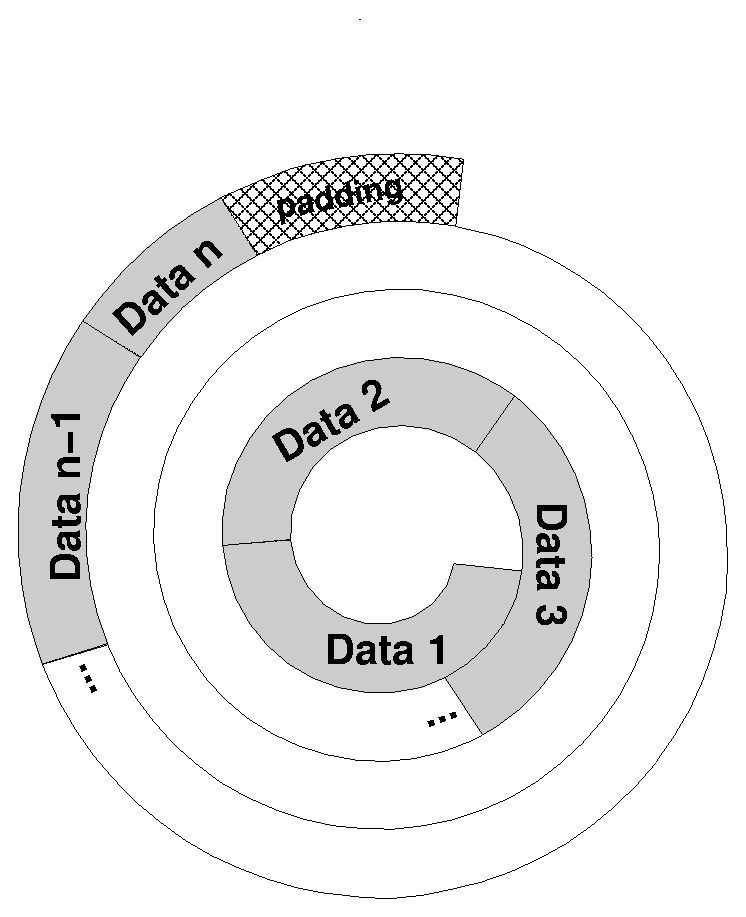
\includegraphics[width=67mm]{spiral-rs01.eps}
 \caption{Interpretation of physical layout in the .iso image}
 \label{layout-phy-one}
 \end{center}
\end{figure}

RS01 is meant to protect data which has already been written to an optical
medium, so the parity data can not be appended to the medium and must instead 
be kept in a separate error correction file. Like all dvdisaster
codecs, RS01 is based on a RS(255,k) Reed-Solomon code with  each
ecc block being comprised of $n$ data bytes and $k$ parity bytes, and
$n+k=255$.

The $n$ data bytes are taken from an iso image generated from the medium.
Reading data directly from the optical drive during encoding would slow down the
process tremendously due to massive random access over the medium, and 
quickly wear out the drive mechanics. However producing the .iso image 
takes one fast linear read, accesses the drive in a way it is designed to be used,
and puts the data on hard disk which can sustain the needed random access I/O.

Reed-Solomon codes
work best when errors are evenly distributed over all ecc blocks.
Therefore the $n$ data bytes used for creating an ecc block must be picked from
locations which are evenly distributed over the medium with a maximum
distance between each data byte pair. To obtain a suitable data distribution,
it is taken  into account that optical media are recorded as a single long 
spiral\footnote{Multiple layered
media contain one spiral for each physical layer, but are otherwise conceptually
identical.} of sectors each containing 2048 bytes.
The first sector lies at the innermost position of the spiral and is indexed with 0;
numbering continues onward to the outside of the spiral. The .iso image
contains a 1:1 mapping of this storage scheme, with the first 2048 bytes
holding the contents of sector 0, the next 2048 bytes resembling sector 1, and so on.

When encoding with $n$ data bytes per ecc block, the iso image is divided into
$n$ layers which physically map to the medium as shown in fig.\ref{layout-phy-one}. 
This distributes the ecc block reasonably good over the medium surface.
However since the image size does not need
to be a multiple of the layer size, the $n$-th layer may be physically shorter
as the layer size. For encoding purposes, the non-existant sectors in layer
$n$ are treated as sectors being filled with 2048 zero bytes. 

\subsection{Logical ecc file layout}

\begin{figure}
 \begin{center}
 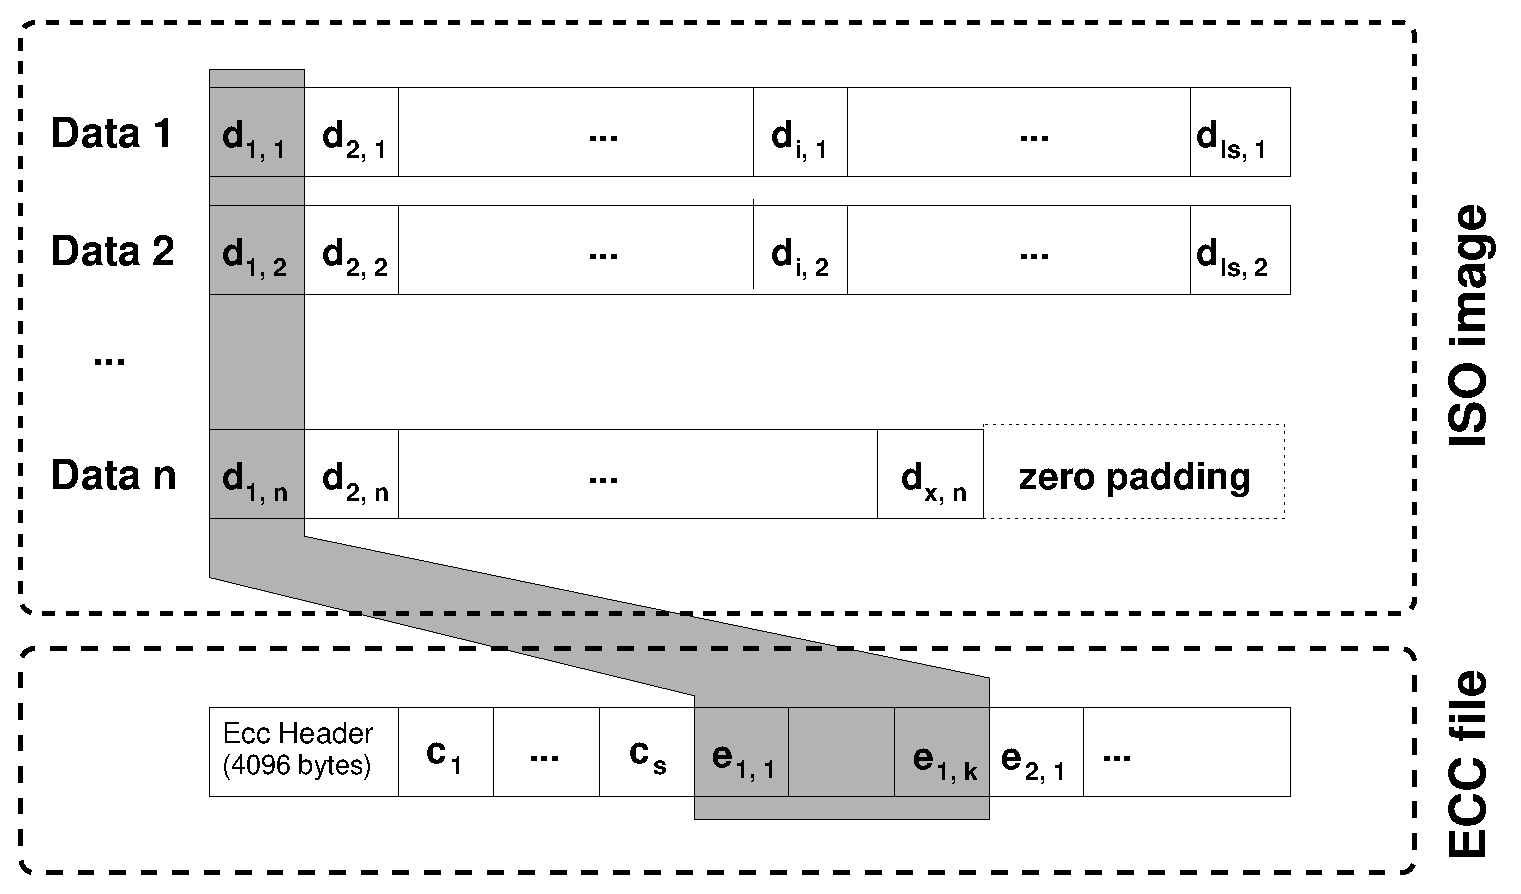
\includegraphics[width=\textwidth]{rs01-layout.eps}
 \caption{Logical RS01 layout}
 \label{layout-logical-one}
 \end{center}
\end{figure}

The ecc file layout, and therefore the relationship between the iso image
contents and the ecc file, is shown in 
figure \ref{layout-logical-one}. The first 4096 bytes of the ecc file
contain the ecc header whose format is described in appendix \ref{eh}.
For RS01, only the data fields marked with ``all'' or ``RS01'' are
relevant; all other fields should be set to zero.

Next to the ecc header comes the CRC section of the ecc file. If the
iso image contains $s$ sectors, the next $4*s$ bytes in the ecc file
contain the CRC32 sums of the sectors from the iso image: Let $b_1,\dots,b_{2048}$ denote 
the bytes of the first data sector; $b_{2049},\dots,b_{4096}$ those of the
second data sector and so on. Then $c_1 = CRC32(b_1,\dots,b_{2048})$,
$c_2 = CRC32(b_{2049},\dots,b_{4096})$ etc. Note that in contrast to
RS02 and RS03, bytes from the CRC section are not included into the ecc block
calculation and are therefore not protected by ecc.

\smallskip

The remainder of the ecc file contains the parity bytes of the
ecc blocks. For an ecc file built with $k$ roots, 
the iso image is logically divided into 
$n = 255-k$ layers as shown in figure \ref{layout-logical-one}.
The $d_{i,j}$ denote the $i-th$ byte in the $j-th$ layer.
In order to create the first ecc block, bytes $d_{1,1}$ to  $d_{1,n}$ are taken from the
$n$ layers. Then the RS(255,k) code is calculated (see appendix \ref{rs} for its parameters)
and the 
resulting $k$ parity bytes $e_{1,1}$ upto $e_{k,1}$ are stored
in the ecc file. The resulting ecc block is marked grey in the
figure. The next ecc blocks are calculated and stored accordingly.
In total, the ecc section contains $k*ls$ bytes of parity information,
with the $k$ parity bytes of each ecc block being stored consecutively.

\subsection{Calculating the layout for encoding}

The RS01 layout is fully determined by the number of roots for the error correction code
and the iso image size in sectors (from now on, ``size'' always means ``number of
2048K sectors). The number of roots can be freely chosen by the user from the
range of $[8...100]$. The iso image size is directly measured
from the iso image file.

\smallskip

The number of data layers is simply calculated from the number of roots, $k$:

\[ data\ layers = 255 - k\]

The size of each layer is:

\[ layer\ size = \left\lceil\frac{medium\ size}{data\ layers}\right\rceil\]

At the end of the last layer, $data\ layers * layer\ size - medium\ size$
zero filled padding sectors are used in the encoding process.

\subsection{Getting the layout when recovering defective media}

The required parameters are taken from the ecc header stored in
the error correction file (see appendix \ref{eh}). Especially,
the number of roots are taken from the {\em eccBytes} field and
the medium size is recorded in the {\em sectors} field.

\subsection{md5 checksums}

RS01 provides two md5 checksums for integrity checking.
The md5 sum of the iso image is calculated and stored in the
{\em mediumSum} field of the ecc header. 
Another md5 sum is calculated over the ecc file, excluding the
first 4096 bytes, and stored in the {\em eccSum} field of
the ecc header. It can be used to verify the integrity of the
ecc file itself. The ecc header is protected by its own CRC
checksum which is stored in the {\em selfCRC} field.

\smallskip

The md5 checksum generation is the major obstacle for parallelizing
the encoder. In RS03, md5sum generation has been made optional since
the RS03 layout allows suffcient consistency checks 
by doing a quick error syndrome check using the Reed-Solomon code.

\subsection{Special cases}

Error correction files can be created for any type of input files, not just iso files,
as long as the input files are ``reasonably'' long\footnote{Input files should contain
at least 2048*(255-k) bytes, so that there is at least one sector for each data
layer.}. Since input files are processed in units of 2048 kByte sectors, 
files whose byte size is not an integer multiple of 2048 are virtually padded 
with zeroes. In that case, the {\em inLast} field of the ecc header
contains the real byte size of the last file ``sector'' so that recovering the
last file sector does not write out the padding bytes. A size of zero in the
{\em inLast} field means that the last sector contains 2048 bytes.
